\documentclass{resume}

\begin{document}

\fontfamily{ppl}\selectfont

\noindent
\begin{tabularx}{\linewidth}{@{}m{0.8\textwidth} m{0.2\textwidth}@{}}
{
    \Large{Dylan Randle} \newline
    \small{
        \clink{
            \href{mailto:dylanrandle@gmail.com}{dylanrandle@gmail.com}
            \textbf{·} 
            \href{https://dylanrandle.github.io/}{dylanrandle.github.io}
        } \newline
        Boston, USA
    }
} & 
{
    \hfill
    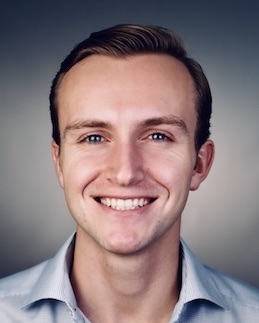
\includegraphics[scale=0.3]{images/headshot.jpg}
}
\end{tabularx}
\begin{center}
\begin{tabularx}{\linewidth}{@{}*{2}{X}@{}}
% left side %
{
    \csection{RELEVANT EXPERIENCE}{\small
        \begin{itemize}
            
            \item \frcontent{Amazon Robotics}{Data Scientist II -- North Reading, MA}{
            	Led development of optimization algorithms for robot path planning. 
		Demonstrated +10\% performance improvement and potential cost savings of \$150M/year.
		Paper accepted for presentation at internal conference (4\% acceptance rate).
		}{July 2020 - Present}
            
            \item \frcontent{Harvard University}{Teaching Fellow -- Cambridge, MA}{
            	Prepared lecture materials on neural networks and tree-based ensemble models.
		Led hands-on lab sessions covering AWS, Hadoop, Spark, OpenMP, MPI.
		Awarded ``Special Distinction in Teaching".
		}{October 2019 - May 2020}
	    
            \item \frcontent{Amazon Robotics}{Data Scientist, Intern -- North Reading, MA}{
            	Designed and developed automated machine learning (AutoML) library for trillion-row datasets.
		Reduced time and complexity of data preparation, model training, and result interpretation.
		}{May 2019 - August 2019}
		
            \item \frcontent{Hubdoc}{Data Scientist -- Toronto, Canada}{
            	Designed, developed, and deployed natural language processing (NLP) system for extracting key information from invoices, bills, and receipts. 
		Served tens of thousands of customer inference requests per day with $\leq 2s$  latency.
		}{February 2017 - July 2018}
		
        \end{itemize}
    }
    \csection{TECHNICAL SKILLS}{\footnotesize
        \begin{itemize}
            \item \textbf{Languages}: Python (numpy, pandas, pytorch, keras), SQL
            \item \textbf{Tools}: Git, Conda, Jupyter, Docker
            \item \textbf{Platforms}: AWS
        \end{itemize}
    }
} 
& 
% right side %
{
  \csection{EDUCATION}{\small
        \begin{itemize}
            
            \item \frcontent{Harvard University}{M.S. Data Science}{
		Thesis: ``Unsupervised Neural Network Methods for Solving Differential Equations".
            }{September 2018 - May 2020}
            
            \item \frcontent{University of California, Berkeley}{B.S. Industrial Engineering \& Operations Research}{
            	Courses: Statistics, Optimization, Machine Learning, Stochastic Processes, Simulation.
            }{September 2012 - May 2016}
            
        \end{itemize}
    }
    \csection{SELECTED PROJECTS}{\footnotesize
        \begin{itemize}
        
        		\item Unsupervised Learning of Solutions to Differential Equations with GANs
		\newline \href{https://dylanrandle.github.io/projects/denn/deqgan.html}{\texttt{dylanrandle.github.io/projects/denn/deqgan.html}}
		
		\item Generating Faces with a ResNet VAE
		\newline \href{https://github.com/dylanrandle/deepgen}{\texttt{github.com/dylanrandle/deepgen}} 
	   
            	\item Learning Interpretable Decision Sets for Healthcare with RL
		\newline \href{https://dylanrandle.github.io/projects/irl/irl.html}{\texttt{dylanrandle.github.io/projects/irl/irl.html}}
		
        \end{itemize}
    }
    
     \csection{RECOGNITIONS}{\footnotesize
        \begin{itemize}
        		\item Special Distinction in Teaching (Harvard University, 2020)
		\item Scholarship in Applied Computation (Harvard University, 2019)
		\item High Honors at Graduation (UC Berkeley, 2016)
		\item Dean’s Honors (UC Berkeley, 2012 - 2016)
		\item Frank Kraft Award (UC Berkeley, 2012)
        \end{itemize}
    }
    
    \csection{CERTIFICATES}{\footnotesize
        \begin{itemize}
        		\item Divide and Conquer, Sorting and Searching, and Randomized Algorithms (Coursera: ZQ5K6VY43UN5)
		\item Graph Search, Shortest Paths, and Data Structures (Coursera: ERUDV3QR9773)
        \end{itemize}
    }
}
\end{tabularx}
\end{center}
\end{document}